\documentclass[1p,16pt]{elsarticle}
\makeatletter
\def\ps@pprintTitle{%
 \let\@oddhead\@empty
 \let\@evenhead\@empty
 \def\@oddfoot{}%
 \let\@evenfoot\@oddfoot}
\makeatother

%% Use the option review to obtain double line spacing
%% \documentclass[authoryear,preprint,review,12pt]{elsarticle}

%% Use the options 1p,twocolumn; 3p; 3p,twocolumn; 5p; or 5p,twocolumn
%% for a journal layout:
%% \documentclass[final,1p,times]{elsarticle}
%% \documentclass[final,1p,times,twocolumn]{elsarticle}
%% \documentclass[final,3p,times]{elsarticle}
%% \documentclass[final,3p,times,twocolumn]{elsarticle}
%% \documentclass[final,5p,times]{elsarticle}
%% \documentclass[final,5p,times,twocolumn]{elsarticle}

%% For including figures, graphicx.sty has been loaded in
%% elsarticle.cls. If you prefer to use the old commands
%% please give \usepackage{epsfig}

%% The amssymb package provides various useful mathematical symbols
\usepackage{amssymb}
\usepackage{amsmath}
\usepackage{graphicx}
\graphicspath{ {./figures/} }
\usepackage[colorlinks]{hyperref}
\hypersetup{citecolor=DeepPink4}
\hypersetup{linkcolor=DarkRed}
\hypersetup{urlcolor=DarkBlue}
\usepackage{hyperref}
\usepackage{subcaption}

%% The amsthm package provides extended theorem environments
%% \usepackage{amsthm}

%% The lineno packages adds line numbers. Start line numbering with
%% \begin{linenumbers}, end it with \end{linenumbers}. Or switch it on
%% for the whole article with \linenumbers.
%% \usepackage{lineno}

\journal{Hardware and Embedded Systems Security}

\begin{document}

\begin{frontmatter}

%% Title, authors and addresses

%% use the tnoteref command within \title for footnotes;
%% use the tnotetext command for theassociated footnote;
%% use the fnref command within \author or \address for footnotes;
%% use the fntext command for theassociated footnote;
%% use the corref command within \author for corresponding author footnotes;
%% use the cortext command for theassociated footnote;
%% use the ead command for the email address,
%% and the form \ead[url] for the home page:
%% \title{Title\tnoteref{label1}}
%% \tnotetext[label1]{}
%% \author{Name\corref{cor1}\fnref{label2}}
%% \ead{email address}
%% \ead[url]{home page}
%% \fntext[label2]{}
%% \cortext[cor1]{}
%% \address{Address\fnref{label3}}
%% \fntext[label3]{}

\title{Assignment 2: Side-Channel Analysis and Fault Injection}

%% use optional labels to link authors explicitly to addresses:
%% \author[label1,label2]{}
%% \address[label1]{}
%% \address[label2]{}

\author{Amar Lakshya (AXX945), Calvin Menezes (CXM1010)}

\address{School of Computer Science, University of Birmingham}

% \begin{abstract}
%
% \end{abstract}
%
% \begin{keyword}
% %% keywords here, in the form: keyword \sep keyword
% %% PACS codes here, in the form: \PACS code \sep code
% %% MSC codes here, in the form: \MSC code \sep code
% %% or \MSC[2008] code \sep code (2000 is the default)
%
% \end{keyword}
%
\end{frontmatter}

%% \linenumbers

%% main text
\section{Task1}
\label{Task1}
\bf{TODO}
\section{Task2}
\label{Task2}
\subsection{Oscilloscope Capture}%
\label{sub:oscilloscope_capture}
The image of the RSA operations can be seen in Fig~\ref{fig:oscilloscope}

\subsection{Manual Extraction}%
\label{sub:manual_extraction}

\subsection{Acquired Trace}%
\label{sub:acquired_trace}

\subsection{SPA}%
\label{sub:spa}

The image of the RSA operations can be seen in Fig~\ref{fig:acquired_trace}

\section{Task3}
\label{Task3}


\bf{TODO}

\section{Task4}
\label{Task4}
\subsection{Fault Injection on RSA-CRT}%
\label{sub:fault_injection_on_rsa_crt}
From the given values
$n=91, e=5, S=48, \overline{S}=35, x=55$
we calculate the valid signature $y$ by:
\begin{align}
	y &= x^e \mod n \\
	y &= 55^5 \mod 91 \\
	y & = 48
\end{align}

\subsubsection{Using Bellcore Method}%
\label{sub:ballcore_method}
The bellcore method gives factor $q$ by:
\begin{align}
	q &= gcd(S - \overline{S}, n) \\
	q &= gcd(48 - 35, 91) \\
	q &= gcd(13, 91) \\
	q &= 13
\end{align}

we know $n = p * q$ therefore factor $p$ is:
\begin{align}
	p &= n / q \\
	p &= 91 / 13 \\
	p &= 7
\end{align}


\subsubsection{Using Lenstra Method}%
\label{sub:lenstra_method}
The Lenstra method gives factor $q$ by:
\begin{align}
	q &= gcd(\overline{Y}^e - x, n) \\
\end{align}

From eq 1, we know that $y=48$ and since
$\overline{y} = y, \overline{y} = 48$, therefore

\begin{align}
	q &= gcd(48^5 - 55, 91) \\
	q &= gcd(48 - 55, 91) \\
	q &= gcd(7, 91) \\
	q &= 7
\end{align}

we know $n = p * q$ therefore factor $p$ is:

\begin{align}
	p &= n / q \\
	p &= 91 / 7 \\
	p &= 13
\end{align}

The major advantage of Lenstra method is that only the faulty value $\overline{S}$ needs to be known.



\subsection{Counter Measures}%
\label{sub:counter_measures}
\bf{TODO}

I am citing this now \cite{commons_stages_2015}.
%% The Appendices part is started with the command \appendix;
%% appendix sections are then done as normal sections
%% \appendix

%% \section{}
%% \label{}

%% If you have bibdatabase file and want bibtex to generate the
%% bibitems, please use
%%
\bibliographystyle{elsarticle-num}
\bibliography{bibliography}


\begin{figure}[hb]
	\centering
    \centerline{\includegraphics[width=8cm]{oscilloscope}}
    \caption{The picture of oscilloscope showing the first 6 operations of RSA}\label{fig:oscilloscope}
\end{figure}

\begin{figure}[hb]
	\centering
    \centerline{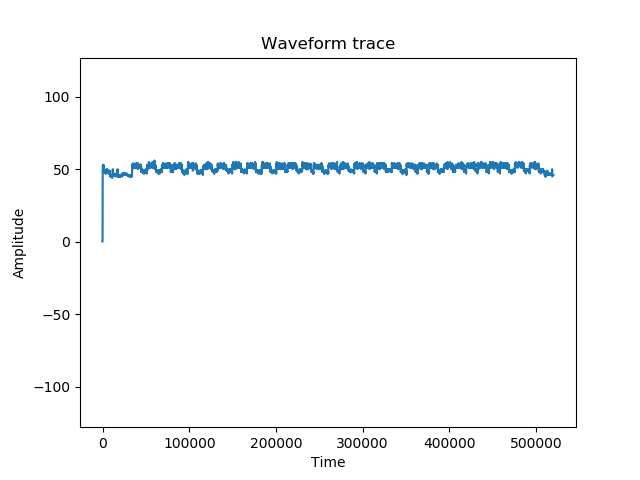
\includegraphics[width=10cm]{trace_plot}}
    \caption{Graph of the acquire trace in full scale}\label{fig:acquired_trace}
\end{figure}

%% else use the following coding to input the bibitems directly in the
%% TeX file.

% \begin{thebibliography}{00}
%
% \bibitem{pizzaOrigins1991} Perry, C. {\em A Stone-Age Snack : History: Pizza topped with tomatoes, pepperoni and cheese is only 100 years old}. Los Angeles Times,1991
% %% Text of bibliographic item%
% \end{thebibliography}
\end{document}
\endinput
%%
%% End of file `elsarticle-template-num.tex'.
